\section{Generating referring expressions} \label{sec:gre}

Now we apply description logic to GRE.  The core claim of this paper
is that it is natural and useful to view the GRE problem as the
problem of computing a formula of description logic whose extension is
a given target set of individuals.

\medskip
\noindent
{\small
\begin{center}
\begin{tabular}{ll} \hline
\multicolumn{2}{l}{
\textsc{$\gL$-GRE Problem}}\\ \hline
\ \ Input: & A model $\gM$ and a set $A \subseteq \Delta^\gM$.\\
\ \ Output: & A formula $\varphi \in \gL$ such that
$\interp{\varphi}^\gM = A$\\ 
& \hspace*{0.5cm} (if such a formula exists).\\ \hline
\end{tabular}
\end{center}}
\medskip

In the examples above, it is because $\mathsf{flower} \sqcap \exists
\mathsf{in}. \mathsf{hat}$ denotes exactly $\{f_2\}$ that we can say
``the flower in the hat'' to refer to $f_2$.  This perspective
provides a general framework into which many existing GRE approaches
fit: Traditional attribute selection \cite{Dale1995} corresponds to
building purely DL formulas that are conjunctions of atoms; relational
REs as in \newcite{dale91:_gener_refer_expres_invol_relat} are
formulas of \el; and so on.  We will pursue the idea of organizing GRE
approaches with respect to the variant of DL they use further in
Section~\ref{sec:related}.

For the rest of this paper, we assume that we are generating a
singular RE, i.e.\ the target referent $A$ will generally be a
singleton set.  In this case, we will only be able to generate a
formula that denotes exactly $A = \{a\}$ (i.e., a RE that uniquely
refers to $a$) if there is no other individual $b$ to which $a$ is
similar; otherwise, any formula that is satisfied by $a$ is also
satisfied by $b$.  Conversely, if we know that $a$ is not similar to
any other individual, then there is a concept that is satisfied by $a$
and not by anything else; this concept can serve as a unique singular
RE.  In other words, we can reduce the $\gL$-GRE problem for a given
model to the problem of computing the $\gL$-similarity sets of this
model.

In the rest of this section, we will present algorithms that compute
the similarity sets of a given model for \alc\ and \el, and for each
similarity set, a characteristic formula that denotes exactly this
set.  In the \alc\ case, we adapt a standard algorithm from the
literature for computing \emph{simulation classes}; we will then
further adapt this algorithm for \el.  In effect, both algorithms
compute REs for all individuals in some model at the same time -- very
efficiently and without any danger of infinite regress.


\begin{figure}[t]
  \centering
  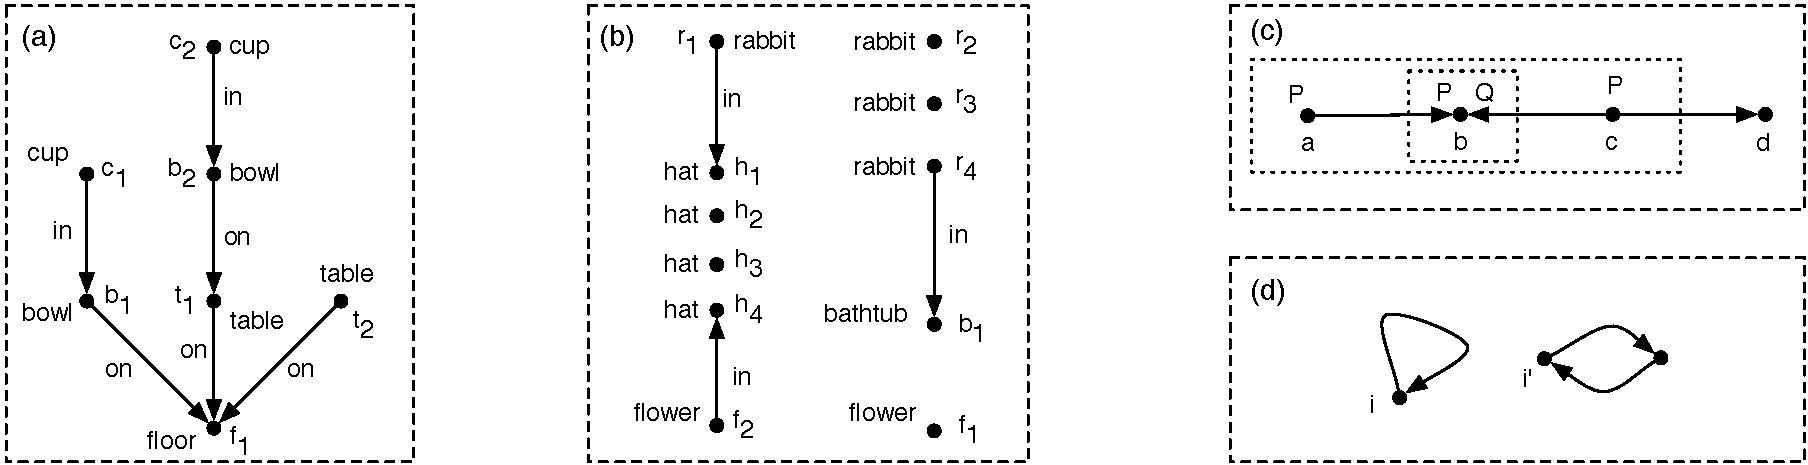
\includegraphics[width=\columnwidth]{pic-dale-haddock}
  \caption{(a) The \newcite{dale91:_gener_refer_expres_invol_relat}
    scenario; (b) the \newcite{Stone1998a} scenario.}
  \label{fig:dale-haddock}
\end{figure}


\subsection{Computing similarity sets}

It can be shown that for \alc, the similarity sets of a finite model
coincide exactly with the \emph{simulation classes} of this model
\cite{blac:moda01}.  We don't have the space here to define simulation
classes, but they have been studied extensively in the literature, and
there are several efficient algorithms for computing \alc-simulation
classes
\cite{hopc:algo71,paig:thre87,dovier04:_effic_algor_for_comput_bisim_equiv}.
However, these algorithms will only compute the simulation classes
themselves. Here we extend the \newcite{hopc:algo71} algorithm such
that it computes, along with each set, also a formula that denotes
exactly this set.  We can then use these formulas as representations
of the REs.

The pseudocode for our \alc\ algorithm is shown as
Algorithm~\ref{algo:bisim-l} and Algorithm~\ref{algo:bisim-add-alc}.
Given a model $\gM=(\Delta, \interp{\cdot})$, the algorithm computes a
set $\RE$ of $\alc$ formulas such that $\{\interp{\varphi} \mid
\varphi \in \RE\}$ is the set of \alc-similarity sets of $\gM$.  The
algorithm starts with $\RE = \{\top\}$ (where $\interp{\top} =
\Delta$), and successively refines $\RE$ by making its elements denote
smaller and smaller sets.  It maintains the invariant that at the
start and end of every iteration, $\{\interp{\varphi} \mid \varphi \in
\RE\}$ is always a partition of $\Delta$.  The algorithm iterates over
all propositional and relational symbols in $\prop$ and $\rel$ to
construct new formulas until either all formulas in $\RE$ denote
singletons (i.e., there is only one individual that satisfies them),
or no progress has been made in the previous iteration.  In each
iteration, it calls the procedure add$_\alc$($\varphi$, $\RE$), which
intersects $\varphi$ with any formula $\psi \in \RE$ which does not
denote a singleton and which is not equivalent to $\varphi$ and to
$\neg \varphi$. In this case, it replaces $\psi$ in $\RE$ by $\psi
\sqcap \varphi$ and $\psi \sqcap \neg \varphi$.



The \alc\ algorithm is capable of computing the \alc-similarity sets
of the model in time $O(nm)$, where $n$ is the number of individuals
in the domain, and $m$ is the number of pairs of individuals that are
related by some relation.  However, it will freely introduce negations
in the case distinctions, which can make the resulting formula hard to
realize (see also Section~\ref{sec:discussion-realization}).  This is
why we also present an algorithm for the \el-similarity sets; \el\
corresponds to positive relational REs, which are generally much
easier to realize.

We obtain the \el\ algorithm by replacing the call to add$_{\alc}$ in
Algorithm~\ref{algo:bisim-l} by a call to add$_{\el}$, which is
defined in Algorithm~\ref{algo:bisim-add-el}.  As before, the
algorithm maintains a set $\RE = \{\varphi_1,\ldots,\varphi_n\}$ of
formulas (this time of \el) such that $\interp{\varphi_1} \cup \ldots
\cup \interp{\varphi_n} = \Delta$, and which it refines iteratively.
However, where the \alc\ algorithm maintains the invariant that
$\interp{\varphi_1},\ldots,\interp{\varphi_n}$ is a partition of
$\Delta$, we weaken this invariant to the requirement that there are
no $m \geq 2$ pairwise different indices $1 \leq i_1,\ldots,i_m \leq
n$ such that $\interp{\varphi_{i_1}} = \interp{\varphi_{i_2}} \cup
\ldots \cup \interp{\varphi_{i_m}}$.  We call the formula
$\varphi_{i_1}$ \emph{subsumed} if such a decomposition exists.

Because it maintains a weaker invariant, the set $\RE$ may contain
more formulas at the same time in the \el\ algorithm than in the \alc\
algorithm.  Prima facie, this means that it has worst-case exponential
runtime, given that the whole domain has an exponential number of
subsets.  However, it is possible that a more careful analysis of the
combinatorics of the considered subsets will reveal that the algorithm
is actually polynomial.

\begin{algorithm}[t]
\dontprintsemicolon
\caption{Computing the $\mathcal{L}$-similarity sets}
\label{algo:bisim-l}
\KwIn{A model $\gM = (\Delta, \interp{\cdot})$}
\KwOut{A set \RE of formulas  such that
$\{\interp{\varphi} \mid \varphi \in \RE\}$ is the set of
$\mathcal{L}$-similarity 
sets of $\gM$.}

$\RE \leftarrow \{\top\}$

\For{$p \in \prop$}{
      add$_\mathcal{L}(p,\RE)$
   }

\While{exists some $\varphi \in \RE, |\interp{\varphi}|^\gM>1$}{
   \For{$\varphi \in \RE, R \in \rel$}{
         add$_\mathcal{L}(\exists R.\varphi,\RE)$
   }
   \If{made no changes to \RE}{
      exit
      }
}
\end{algorithm}

Notice that both algorithms try to refine $\RE$ first according to the
propositional symbols, and then by relational expressions of
increasing depth.  The algorithms would remain correct if we
interleaved the addition of propositional and relational symbols;
however, the algorithms would become slower because the propositional
refinements would have to be percolated through the relational chains
in subsequent iterations.



\subsection{Some examples}\label{sec:examples}

We will now see what our algorithms do for some interesting
examples. Consider the model shown in Fig.~\ref{fig:dale-haddock}a,
which is taken from \newcite{dale91:_gener_refer_expres_invol_relat},
and let's run the $\el$ algorithm.



\begin{algorithm}[t]
\caption{add$_\alc(\varphi,\RE)$}
\label{algo:bisim-add-alc}
\For{$\psi \in \RE$ with $|\interp{\psi}| > 1$}{
   \If{$\interp{\psi \sqcap \varphi} \not = \emptyset$ and
       $\interp{\psi \sqcap \neg \varphi} \not = \emptyset$}{
         add $\psi \sqcap \varphi$ and
               $\psi \sqcap \neg \varphi$ to \RE \;
         remove $\psi$ from \RE \;
      }
   }
\end{algorithm}
%
\begin{algorithm}[t]
\dontprintsemicolon
\caption{add$_\el$($\varphi$, $\RE$)}
\label{algo:bisim-add-el}
\For{$\psi \in \RE$ with $|\interp{\psi}| > 1$}{
  \If{$\psi \sqcap \varphi$ is not subsumed in $\RE$ {\bf and}
    $\interp{\psi \sqcap \varphi} \neq \emptyset$ {\bf and}
    $\interp{\psi \sqcap \varphi} \neq \interp{\psi}$}{
    add $\psi \sqcap \varphi$ to $\RE$ \;
    remove subsumed formulas from $\RE$\;
  }
}
\end{algorithm}

The algorithm starts with $\RE = \{\top\}$.  In the first loop, it
adds the formulas $\mathsf{floor}$, $\mathsf{bowl}$, $\mathsf{cup}$,
and $\mathsf{table}$, and then removes $\top$ because it is now
subsumed.  Not all of these formulas denote singletons; for instance,
$\interp{\mathsf{cup}}$ contains two individuals.  So we iterate over
the relations to refine our formulas.  After the first iteration over
the relations, we have $\RE = \{ \mathsf{floor}, \mathsf{bowl} \sqcap
\exists \mathsf{on}.\mathsf{floor}, \mathsf{bowl} \sqcap \exists
\mathsf{on}.\mathsf{table}, \mathsf{cup}, \mathsf{table} \}$. Notice
that $\mathsf{bowl}$ has become subsumed, but we haven't distinguished
the cups and tables further.

Now we can use the split between the bowls to distinguish the cups in
the second iteration.  The result of this is $\RE = \{ \mathsf{floor},
\mathsf{bowl} \sqcap \exists \mathsf{on}.\mathsf{floor}, \mathsf{bowl}
\sqcap \exists \mathsf{on}.\mathsf{table}, \mathsf{cup} \sqcap \exists
\mathsf{in}. (\mathsf{bowl} \sqcap \exists
\mathsf{on}.\mathsf{floor}), \mathsf{cup} \sqcap \exists
\mathsf{in}. (\mathsf{bowl} \sqcap \exists
\mathsf{on}.\mathsf{table}), \mathsf{table} \}$.  At this point, all
formulas except $\mathsf{table}$ denote singletons, and further
iterations don't allow us to refine $\mathsf{table}$; so the algorithm
terminates.  Each formula with a singleton extension $\{a\}$ is a
unique description of $a$; for instance, $\mathsf{cup} \sqcap \exists
\mathsf{in}. (\mathsf{bowl} \sqcap \exists
\mathsf{on}.\mathsf{table})$ is only satisfied by $c_2$, so we may
refer to $c_2$ as ``the cup in the bowl on the table''.  Notice that
the algorithm didn't focus on any particular individual; it
simultaneously generated REs for all individuals except for the two
tables (which are similar to each other).

The \el\ algorithm has a harder time with the example in
Fig.~\ref{fig:dale-haddock}b \cite{Stone1998a}.  While it will
correctly identify $r_1$ as ``the rabbit in the hat'' and $f_2$ as
``the flower in the bathtub'', it will not be able to compute a RE for
$f_1$ because $f_2$ is \el-similar to $f_1$.  Indeed, the algorithm
terminates with $\RE$ containing both $\mathsf{flower}$ and
$\mathsf{flower} \sqcap \exists \mathsf{in}.\mathsf{hat}$.  This is a
typical pattern for asymmetrical cases of similarity in \el: If there
are two formulas $\varphi_1$ and $\varphi_2$ in the output set with
$\interp{\varphi_1} \subseteq \interp{\varphi_2}$, then there is
generally some individual $b \in \interp{\varphi_2} -
\interp{\varphi_1}$ such that all individuals in $\interp{\varphi_1}$
are similar to $b$, but not vice versa.  By contrast, the \alc\
algorithm can exploit the greater expressivity of \alc\ to split
$\mathsf{flower}$ into the two new formulas $\mathsf{flower} \sqcap
\exists \mathsf{in}.\mathsf{hat}$ and $\mathsf{flower} \sqcap \neg
\exists \mathsf{in}.\mathsf{hat}$, generating a unique RE for $f_1$ as
well.





%%% Local Variables: 
%%% mode: latex
%%% TeX-master: "dl-gre-08"
%%% End: 
